
On dispose d'un pavé droit dont les
  dimensions sont indiquées sur la figure ci-contre. On {\em extrait}
  de ce pavé droit une pyramide ${\cal P}_1$.
  
\begin{center}
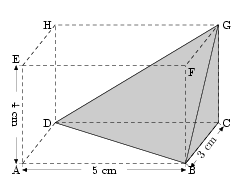
\includegraphics[scale=1]{RepS-25.png}
\end{center}

\begin{enumerate}
  \item Donne la nature {\em la plus précise possible} des faces de cette pyramide.
  \item Construis un patron de cette pyramide.
\end{enumerate}
